\documentclass[12pt,fleqn]{article}\usepackage{../../common}
\begin{document}
Beklenti, Varyans, Kovaryans ve Korelasyon

Beklenti (Expectation) 

Bu değer, dağılım $f(x)$'in tek sayılık bir özetidir. Yani beklenti hesabına
bir taraftan bir dağılım fonksiyonu girer, diğer taraftan tek bir sayı
dışarı çıkar. 

Tanım

Sürekli dağılım fonksiyonları için $E(X)$

$$  E(X) = \int x f(x) \ud x$$

ayrıksal dağılımlar için

$$ E(X) = \sum_x xf(x) $$

Hesabın, her $x$ değerini onun olasılığı ile çarpıp topladığına dikkat. Bu
tür bir hesap doğal olarak tüm $x$'lerin ortalamasını verecektir, ve
dolaylı olarak dağılımın ortalamasını hesaplayacaktır. Ortalama $\mu_x$
olarak ta gösterilebilir.

$E(X)$'in bir tanım olduğuna dikkat, yani bu ifade tamamen bizim
yarattığımız, ortaya çıkarttığımız bir şey, matematiğin baz kurallarından
gelerek türetilen bir kavram değil. Notasyonel basitlik için üstteki toplam
/ entegral yerine

$$ = \int x \ud F(x) $$

diyeceğiz, bu notasyonel bir kullanım sadece, unutmayalım, reel analizde
$\int x \ud F(x)$'in özel bir anlamı var (hoca tam diferansiyel $dF$'den
bahsediyor) [2, sf. 69]. 

Beklentinin tanımının kapsamlı / eksiksiz olması için $E(X)$'in
``mevcudiyeti'' için de bir şart tanımlamak gerekir, bu şart şöyle olsun, 

$$ \int_x |x|dF_X(x) < \infty $$

işe beklenti mevcut demektir. Tersi sözkonusu ise beklenti mevcut
değildir. 

Örnek 

$$
X \sim Unif(-1,3)
$$

olsun.

$$
E(X) = \int x \ud F(x) = \int x f_X(x) \ud x
= \frac{1}{4} \int _{ -1}^{3} x \ud x = 1
$$

Örnek 

Cauchy dağılımının $f_X(x) = \{ \pi (1+x^2) \} ^{-1}$ olduğunu
söylemiştik. Şimdi beklentiyi hesaplayalım. Parçalı entegral tekniği lazım,
$u=x$, $dv = 1/1+x^2$ deriz, ve o zaman $v = \tan ^{-1}(x)$ olur, bkz
[6]. Demek ki

$$
\int |x| \ud F(x)
= \frac{ 2}{\pi} \int _{ 0}^{\infty}\frac{x \ud x}{1+x^2}
$$

2 nereden çıktı? Çünkü $|x|$ kullanıyoruz, o zaman sınır değerlerinde
sadece sıfırın sağına bakıp sonucu ikiyle çarpmak yeterli. Bir sabit olduğu
için $\pi$ ile beraber dışarı çıkıyor. Şimdi

$$ \int udv = uv - \int vdu $$

üzerinden

$$ = [x \tan ^{-1}(x) ] _{ 0}^{\infty} - \int _{ 0}^{\infty} \tan ^{-1}(x)
dx  = \infty$$

Yani üstteki hesap sonsuzluğa gider. O zaman üstteki tanımımıza göre Cauchy
dağılımının beklentisi yoktur. 

$Y$ rasgele değişkeninin varyansı (variance) 

Ayrısak olarak diyelim ki her biri $p_j$ olasılığa sahip $n$ tane değer
$y_i$ arasından, ve beklenti $E(Y) = \mu$ ise, varyans bir tür ``yayınımın
ortalamasıdır''. Yani ortalama olarak ortalamadan (!) ne kadar sapılır
sorusunun cevabını verir,

$$ Var(Y) = \sum _{i=1}^{n}(y_i-\mu)^2 p_i$$

Kare alma işlemi yapıldı çünkü sapmanın eksi mi artı mı olduğu bizi
ilgilendirmiyor, sadece onun mutlak değeri, büyüklüğü bizi
ilgilendiriyor. $p_i$ ile çarptık çünkü mesela bazı sapmaların değeri büyük
olabilir, ama eğer o sapmaların ortaya çıkma olasılığı düşük ise bu
sapmalar toplama, yani varyansa, daha az etki edecektir. Değerlerin $p_i$
ile çarpılıp sonuçların toplanması beklenti hesabını çağrıştırabilir, ve
evet, matematiksel olarak varyans bir tür beklenti hesabıdır. O sebeple
genel bir şekilde alttaki gibi belirtilir,

$$ Var(Y) = E((Y-E(Y))^2) $$

İfadede toplama ve bölme gibi işlemler olmadığına dikkat; onun yerine kare
ifadeleri üzerinde beklenti ifadesi var. Yani $Y$'nin beklentisini rasgele
değişkenin kendisinden çıkartıp kareyi alıyoruz, ve bu işlemin $Y$'den
gelen tüm zar atışları üzerinden beklentisi bize varyansı veriyor. Bir
rasgele değişken görünce onun yerine ``dağılımdan üretilen sayı'' düşünmek
faydalıdır, ki bu gerçek dünya şartlarından (ve büyük miktarda olunca) veri
noktalarını temsil eder. 

Varyans formülünü açarsak, ileride işimize yarayacak başka bir formül elde
edebiliriz, 

$$ Var(Y) = E( Y^2  - 2YE(Y) + (E(Y)^2) )$$

$$  = E(Y^2)  - 2E(Y)E(Y) + (E(Y)^2)$$

$$ Var(Y) = E(Y^2) - (E(Y)^2)$$

Tanım

$y_1,..,y_n$ örnekleminin varyansı (literatürde $S^2$ olarak geçebiliyor,

$$ 
S^2 = 
\frac{1}{n} \sum (y_i - \bar{y})^2
\mlabel{2}
$$

Standart sapma veri noktaların "ortalamadan farkının ortalamasını"
verir. Tabii bazen noktalar ortalamanın altında, bazen üstünde olacaktır,
bizi bu negatiflik, pozitiflik ilgilendirmez, biz sadece farkla
alakalıyız. O yüzden her sapmanın karesini alırız, bunları toplayıp nokta
sayısına böleriz. 

İlginç bir cebirsel işlem şudur ve bize verinin üzerinden tek bir kez
geçerek (one pass) hem sayısal ortalamayı hem de sayısal varyansı
hesaplamamızı sağlar. Eğer $\bar{y}$ tanımını üstteki formüle sokarsak,

$$ = \frac{ 1}{n} \sum_i y_i^2 + \frac{ 1}{n} \sum_i m^2 - \frac{ 2}{n} \sum_i y_i\bar{y}  $$

$$ = \frac{ 1}{n} \sum_i y_i^2 + \frac{ \bar{y}^2n}{n} - \frac{ 2\bar{y}n}{n}\bar{y} $$

$$ = \frac{ 1}{n} \sum_i y_i^2 +  \bar{y}^2 - 2\bar{y}^2 $$

$$ = \frac{ 1}{n} \sum_i y_i^2 - \bar{y}^2 $$

ya da 

$$ = \sum _{i=1}^{n} y_i^2 - \frac{1}{n} \bigg( \sum _{i=1}^{n} y_i \bigg)^2  
\mlabel{5}
$$

Bu arada standard sapma varyansın kareköküdür, ve biz karekök olan versiyon
ile çalışmayı tercih ediyoruz. Niye? Çünkü o zaman veri noktalarının ve
yayılma ölçüsünün birimleri birbiri ile aynı olacak. Eğer veri setimiz bir
alışveriş sepetindeki malzemelerin lira cinsinden değerleri olsaydı,
varyans bize sonucu "kare lira" olarak verecekti ve bunun pek anlamı
olmayacaktı.

Kovaryans ve Korelasyon

Harvard Joe Blitzstein dersinden alınmıştır

Bugün ``kovaryans günü'', bu tekniği kullanarak nihayet bir toplamın
varyansını bulabileceğiz, varyans lineer değildir (kıyasla beklenti
-expectation- lineerdir). Bu lineer olmama durumu bizi korkutmayacak tabii,
sadece yanlış bir şekilde lineerlik uygulamak yerine probleme farklı bir
şekilde yaklaşmayı öğreneceğiz. 

Diğer bir açıdan, hatta bu ana kullanımlardan biri, kovaryans iki rasgele
değişkeni beraber / aynı anda analiz etmemize yarayacak. İki varyans
olacak, ve onların alakasına bakıyor olacağız, bu sebeple bu analize {\em
  ko}varyans deniyor zaten. 

Tanım

$$ 
Cov(X,Y) = E((X-E(X))(Y-E(Y))) 
\mlabel{1} 
$$

Burada $X,Y$ aynı uzayda tanımlanmış herhangi iki rasgele değişken. Üstteki
diyor ki rasgele değişken $X,Y$'in kovaryansı $X$'ten ortalaması
çıkartılmış, $Y$'ten ortalaması çıkartılmış halinin çarpılması ve tüm bu
çarpımların ortalamasının alınmasıdır.

Tanım böyle. Şimdi bu tanıma biraz bakıp onun hakkında sezgi / anlayış
geliştirmeye uğraşalım. Tanım niye bu şekilde yapılmış, başka bir şekilde
değil?

İlk önce eşitliğin sağ tarafındaki bir çarpımdır, yani ``bir şey çarpı bir
başka şey''. Bu ``şeylerden'' biri $X$ ile diğeri $Y$ ile alakalı, onları
çarparak ve çarpımın bir özelliğinden faydalanarak şunu elde ettik; artı
çarpı artı yine artı değerdir, eksi çarpı artı eksidir, eksi çarpı eksi
artıdır. Bu şekilde mesela ``aynı anda artı'' olmak gibi kuvvetli bir
bağlantı çarpımın artı olması ile yakalanabilecektir. Aynı durum eksi, eksi
de için geçerli, bu sefer her iki rasgele değişken aynı şekilde
negatiftir. Eksi çarpım sonucu ise sıfırdan az bir değerdir, ``kötü
korelasyon'' olarak alınabilir ve hakikaten de eksi artı çarpımının işareti
olduğu için iki değişkenin ters yönlerde olduğunu gösterir. Demek ki bu
araç / numara hakikaten faydalı.

Unutmayalım, üstteki çarpımlardan birisinin büyüklüğü $X$'in ortalamasına
bağlı olan bir diğer, $Y$ aynı şekilde. Şimdi $X,Y$'den bir örneklem
(sample) aldığımızı düşünelim. Veri setinin her veri noktası bağımsız
özdeşçe dağılmış (i.i.d) durumda. Yani $X,Y$ değişkenlerine ``gelen''
$x_i,y_i$ ikilileri her $i$ için diğerlerinden bağımsız; fakat her ikilinin
arasında bir bağlantı var, yani demek ki bu rasgele değişkenlerin baz
aldığı dağılımların bir alakası var, ya da bu iki değişkenin bir ortak
dağılımı (joint distribution) var.

Not: Eğer $X,Y$ bağımsız olsaydı, o zaman 

$$ Cov(X,Y) = E((X-E(X))) E(Y-E(Y))  $$

olarak yazılabilirdi, yani iki beklentinin ayrı ayrı çarpılabildiği
durum... Ama biz bu derste bağımsızlığın olmadığı durumla ilgileniyoruz..

Korelasyon kelimesinden bahsedelim hemen, bu kelime günlük konuşmada çok
kullanılıyor, ama bu ders bağlamında korelasyon kelimesinin matematiksel
bir anlamı olacak, onu birazdan, kovaryans üzerinden tanımlayacağız.

Bazı ilginç noktalar:

Özellik 1

varyansı nasıl tanımlamıştık? 

$$ Var(X) = E( (X-E(X))^2 )  $$

Bu denklem aslında 

$$ Cov(X,Y) = E( (X-E(X))(Y-E(Y)) )  $$

denkleminde $Y$ yerine $X$ kullandığımızda elde ettiğimiz şeydir, yani

$$ Cov(X,X) = E((X-E(X))(X-E(X)))  $$

$$ Cov(X,X) = E((X-E(X))^2)   $$

$$ = Var(X) $$

Yani varyans, bir değişkenin ``kendisi ile kovaryansıdır''. İlginç değil
mi? 

Özellik 2

$$ Cov(X,Y) = Cov(Y,X) $$

İspatı kolay herhalde, (1) formülünü uygulamak yeterli.

Teori

$$ Cov(X,Y) = E((X-E(X))(Y-E(Y))) = E(XY) - E(X)E(Y)$$

İspat

Bu ispat çok kolay, eşitliğin sol tarafındaki çarpımı parantezler üzerinden
açarsak, ve beklenti lineer bir operatör olduğu için toplamın terimleri
üzerinde ayrı ayrı uygulanabilir, 

$$ E(XY) -E(X)E(Y) -E(X)E(Y) + E(X)E(Y) $$

$$  =  E(XY) - E(X)E(Y) $$

Çarpımı uygularken mesela $E(-X \cdot E(Y))$ gibi bir durum ortaya çıktı,
burada $E(Y)$'nin bir sabit olduğunu unutmayalım, çünkü beklenti rasgele
değişkene uygulanınca tek bir sayı ortaya çıkartır, ve vu $E(Y)$ üzerinde
bir beklenti daha uygulanınca bu ``içerideki'' beklenti sabitmiş gibi
dışarı çıkartılabilir, yani $-E(X)E(Y)$. 

Devam edelim, $E(XY) - E(X)E(Y)$ ifadesini gösterdik, çünkü çoğu zaman bu
ifade hesap açısından (1)'den daha uygundur. Ama (1) ifadesi anlatım /
sezgisel kavrayış açısından daha uygun, çünkü bu ifade $X$'in ve $Y$'nin
kendi ortalamalarına izafi olarak belirtilmiştir, ve akılda canlandırılması
daha rahat olabilir. Fakat matematiksel olarak bu iki ifade de aynıdır. 

İki özellik bulduk bile. Bir özellik daha,

Özellik 3

$$ Cov(X,c) = 0 $$

Bu nereden geldi? (1)'e bakalım, $Y$ yerine $c$ koymuş olduk, yani bir
sabit. Bu durumda (1)'in $(Y-E(Y))$ kısmı $c-E(c)=c-c=0$ olur [aslında
bayağı absürt bir durum], ve bu durumda (1) tamamen sıfıra dönüşür, sonuç sıfır.

Özellik 4

$Cov(cX,Y) = c \cdot Cov(X,Y)$ 

İspat için alttaki formülde

$$ Cov(X,Y) =  E(XY) - E(X)E(Y) $$

$X$ yerine $cX$ koymak yeterli, $c$ her iki terimde de dışarı çıkacaktır,
ve grubun dışına alıncan bu özelliği elde ederiz.

Özellik 5

$$ Cov(X,Y+Z) = Cov(X,Y) + Cov(X,Z) $$

İspat için bir üstteki özellikte yaptığımızın benzerini yaparız. 

En son iki özellik oldukça faydalıdır bu arada, onlara ikili-lineerlik
(bilinearity) ismi veriliyor. İsim biraz renkli / sükseli bir isim,
söylemek istediği şu aslında, bu son iki özellikte sanki bir kordinatı
sabit tutup diğeri ile işlem yapmış gibi oluyoruz, yani bir kordinat sabit
olunca diğeri ``lineermiş gibi'' oluyor; Mesela $c$'nin dışarı çıktığı
durumda olduğu gibi, bu özellikte $Y$'ye hiçbir şey olmadı, o değişmeden
kaldı. Aynı şekilde 5. özellikte $X$ hiç değişmeden eşitliğin sağına
aktarıldı sanki, sadece ``$Z$ durumu için'' yeni bir terim ekledik. 

4. ve 5. özellik çok önemlidir, bunları bilirsek bir ton hesabı yapmadan
hızlıca türeterek hesaplar kolaylaştırılabilir.

Özellik 6

$$ Cov(X+Y, Z+W) = Cov(X,Z) + Cov(X,W) + Cov(Y,Z) + Cov(Y,W) $$

Şimdi 5. özelliği hatırlayalım, orada gösterilen sanki bir nevi basit
cebirdeki dağıtımsal (distributive) kuralın uygulanması gibiydi sanki, yani
$(a+b)(c+d)$'i açtığımız gibi, 5. özellik te sanki kovaryansı çarpıp
topluyormuş gibi ``açıyordu''. En temelde gerçekten olan bu değil ama nihai
sonuç benzer gözüktüğü için akılda tutması kolay bir metot elde etmiş
oluyoruz. Her neyse, 6. özellik için aslında 5. özelliği tekrar tekrar
uygulamak yeterli. Bu arada 5. özellik $Cov(X,Y+Z)$ için ama $Cov(Y+Z,X)$
yine aynı sonucu veriyor. 

Bu arada 6. özellik çok çetrefil toplamlar üzerinde de uygulanabilir,
mesela 

$$ Cov \bigg( \sum _{i=1}^{m}a_iX_i, \sum _{j=1}^{n}b_iY_i \bigg) $$

Bu son derece karmaşık gözüküyor, fakat çözümü için aynen 6. özellikte
olduğu gibi 5. özelliği yine tekrar tekrar uygulamak yeterli (4. özellik
ile de sabiti dışarı çıkarırız, vs).

Çoğu zaman üstteki gibi pür kovaryans içeren bir açılımla çalışmak, içinde
beklentiler olan formüllerle uğraşmaktan daha kolaydır. 

Şimdi toplamlara dönelim; kovaryanslara girmemizin bir sebebi toplamlarla
iş yapabilmemizi sağlaması. Mesela, bir toplamın varyansını nasıl
hesaplarız? 

Özellik 7

$$ Var(X_1+X_2) $$

Şimdilik iki değişken, ama onu genelleştirip daha fazla değişkeni
kullanabiliriz. 

Çözelim. 1. özellik der ki varyans değişkenin kendisi ile kovaryansıdır,
yani $Var(X) = Cov(X,X)$. O zaman $Var(X_1+X_2) = Cov(X_1+X_2,
X_1+X_2)$. Böylece içinde toplamlar içeren bir kovaryans elde ettik ama bunu çözmeyi 
biliyoruz artık. ``Dağıtımsal'' işlemleri yaparken $Cov(X_1,X_1)$ gibi
ifadeler çıkacak, bunlar hemen varyansa dönüşecek. Diğer taraftan
$Cov(X_1,X_2)$ iki kere gelecek, yanı

$$ Var(X_1+X_2) = Var(X_1) + Var(X_2)  + 2 Cov(X_1,X_2)$$

Bu alanda bilinen tekerleme gibi bir başka deyiş, ``eğer kovaryans sıfırsa
toplamın varyansı varyansların toplamıdır''. Hakikaten kovaryans sıfır
olunca üstteki denklemden düşecektir, geriye sadece varyansların toplamı
kalacaktır. Kovaryans ne zaman sıfırdır? Eğer $X_1,X_2$ birbirinden
bağımsız ise. Tabii bu bağımsızlık her zaman ortaya çıkmaz. 

İkiden fazla değişken olunca? Yine tüm varyansların ayrı ayrı toplamı, ve
kovaryanslar da sonda toplanacak,

$$ Var(X_1+ .. + X_n ) = Var(X_1) + .. + Var(X_n) + 2 \sum _{i<j}^{} Cov(X_i,X_j) $$

Sondaki toplamın indisinde bir numara yaptık, sadece 1 ile 2, 2 ile 3,
vs. eşlemek için, ve mesela 3 ile 1'i tekrar eşlememek için. Tekrar dedik
çünkü $Cov(X_1,X_3) = Cov(X_3,X_1)$. Eğer indisleme numarası
kullanmasaydık, 2 ile çarpımı çıkartırdık (ona artık gerek olmazdı),

$$ ..  + \sum _{i \ne j} Cov(X_i,X_j) $$

Şimdi, korelasyon konusuna gelmeden önce, bağımsızlık kavramını iyice
anladığımızdan emin olalım. 

Teori

Eğer $X,Y$ bağımsız ise bu değişkenler bağımsızdır, yani $Cov(X,Y)=0$.

DİKKAT! Bu mantık çizgisinin tersi her zaman doğru olmayabilir, yani
bağımsızlık kesinlikle $Cov(X,Y)=0$ demektir, ama her $Cov(X,Y)=0$ olduğu
zaman ortada bir bağımsızlık var diyemeyiz. Bunu bir örnekle görelim. 

$$ Z \sim N(0,1), X=Z, Y=Z^2 $$

Şimdi $X,Y$ kovaryansının hesabı yapalım

$$ Cov(X,Y) = E(XY) - E(X)E(Y) = E(Z^3) - E(Z)E(Z^2)$$

En sondaki terim sıfırdır, çünkü hem $E(Z)$ ve $E(Z^3)$ sıfırdır [hoca
burada standart normalin tek sayılı (odd) moment'leri hep sıfırdır dedi]. O
zaman şu sonucu çıkartıyoruz, $X,Y$ arasında korelasyon yok. 

Ama bağımlılık var mı? Var. Çünkü hem $X$ hem $Y$ $Z$'nin birer değişkeni,
yani bu durumda $X$'i bilmek bize $Y$'yi tamamen bilmemizi sağlıyor (sadece
ek olarak bir kare alıyoruz). Tabii bağımlılık illa herşeyin bilinmesi
demek değildir, biraz bağımlılık ta olabilir, ama biraz bağımlılık bile
varsa, bağımsızlık var diyemeyiz. Aynı şey ters yön için de geçerli, $Y$
bilinince $X$'in ``büyüklüğünü'' bilebiliriz, karekök işlemi olduğu için
-/+ işareti bilemeyiz ama skalar bir büyüklüğü elde edebiliriz. Yani ters
yönde de bağımsızlık yoktur. 

Faydalı bir Eşitlik [1, sf 120]

$$ Var(aX+b) = a^2Var(X) $$

Ya da $b=0$ olduğu durumda (hatta ne olursa olsun)

$$ Var(aX) = a^2Var(X) $$

İspat

$\mu = E(X)$ olsun ve  $E(aX + b) = a\mu + b$ olduğunu hatırlayalım. 
Varyans tanımından hareketle, 

$$ Var(aX+b) = E\big[ (aX + b - E[aX+b] )^2 \big] $$

$$ =  E\big[ (aX + b - a\mu + b )^2 \big]  $$

$$ =  E\big[ (aX - a\mu  )^2 \big]  $$

$$ =  E\big[ a^2(X - \mu)^2 \big]  $$

$$ =  a^2 E\big[ (X - \mu) \big]  $$

$$ =  a^2 Var(X) $$


Korelasyon

Tanım

$$ Corr(X,Y) = \frac{Cov(X,Y)}{SD(X)SD(Y)} 
\mlabel{2}
$$

Bu arada hatırlarsak üstte SD ile gösterilen standart sapma, varyansın
karesidir. 

Bu tanım genelde kullanılan tanımdır. Fakat ben daha farklı bir tanımı
tercih ediyorum. Standardize etmeyi hatırlıyoruz değil mi? Bir rasgele
değişkenden ortalamasını çıkartıp standart sapmaya bölünce standardize
ediyorduk. Bunu kullanarak aslında korelasyonu alttaki gibi
tanımlayabiliriz, 

$$ Corr(X,Y) = Cov \bigg( \frac{X-E(X)}{SD(X)}, \frac{Y-E(Y)}{SD(Y)}
\bigg) 
\mlabel{3}
$$

Yani korelasyonun anlamı aslında şudur: $X,Y$ değişkenlerini standardize
et, ondan sonra kovaryanslarını al (üstteki ifadeye Pearson korelasyonu
ismi de verilir).

Niye standardize edilmiş kovaryans içeren ifadeyi tercih ediyoruz? Çünkü,
diyelim ki $X,Y$ değişkenleri bir uzaklık ölçüsünü temsil ediyor, ve
birimleri mesela nanometre. Fakat bir başkası gelip aynı ölçümü, atıyorum,
ışık yılı olarak kullanmaya başlarsa problem çıkabilir. Yani eğer birim
yoksa ve ben ``$X,Y$ korelasyonum 42'' dersem, bunun ne olduğunu anlamak
zordur. 42 önümüzdeki veriye göre küçük müdür, büyük müdür? Bilemeyiz. Yani
42 sayısı tabii ki evrendeki tüm soruların cevabıdır [hoca bir filme atfen
espri yapıyor, orada 42 sayısının özel bir anlamı vardı], ama önümüzdeki
problem için, nedir?

Fakat üstteki formül ölçü birimsiz (dimensionless) bir sonuç verir, yani
bir ölçü biriminden bahsetmeden birine rahatça aktarabileceğimiz bir
bilgidir. Niye birimsiz oldu? Çünkü $X$'in birimi $cm$ olsa, $X-E(X)$ yine
$cm$, $SD(X)$ varyansın karekökü olduğu için $cm^2$'nin karekökü yine $cm$,
$cm$ bölü $cm$ birim ortadan kalkar.

Bu arada (3) niye (2) ile aynıdır? Eğer bir rasgele değişkenden bir sabiti
çıkartırsam onun başka bir değişken ile kovaryansını değiştirmiş olmam. Ki
standardize etme işlemi bunu yapar. O zaman niye bu çıkartma işlemini
yaptım? Çünkü standardize etme işlemini özellikle kullanmak istedim -
standardizasyon bilinen ve rahatça kullanılabilen bir işlem. Standart
sapmayı bölmeye gelirsek, şimdiye kadar gördüğümüz özelliklerden biri,
bölümü dışarı alabileceğimizi gösteriyor, böyle olunca (2) ifadesini aynen
elde ediyorum. 

Önemli bir nokta daha: korelasyon her zaman $-1$ ve $+1$ arasındadır. 

Teori

$$ -1 \le Corr(X,Y) \le 1 $$

Yani ölçü biriminden bağımsız olması avantajına ek olarak hep aynı skalada
olan bir değerin rapor edilmesi de faydalıdır. Eğer korelasyon 0.99
bulursam bunun hemen yüksek bir korelasyon olduğunu bilirim. 

Bu arada, Çauchy-Schwarz eşitsizliğinden bahsedeyim -ki bu eşitsizlik
tanımı tüm matematikteki en önemli eşitsizliklerden biridir- eğer
korelasyon formülünü lineer cebirsel şekilde ifade etseydim direk
Cauchy-Schwarz eşitsizliğini elde ederdim. 

İspat

Önce ``WLOG çerçevesinde'' $X,Y$'nin önceden standardize edilmiş olduğunu
kabul edelim. [WLOG ne demek? Matematikçiler ispatlar sırasında bunu bazen
kullanırlar, genelleme kuvvetinde bir kayıp olmadan (without loss of
generality) takip eden şeyi kullanabiliriz demektir, yani ``bir başka şey
kullanıyorum, ama teori bu çerçevede de hala geçerli'' demek isterler]. 

Önceden standardize edildiğini kabul etmek niye fark yaratmıyor? Çünkü bunu
gördük, standart olmayan değişkenleri standardize edince yine aynı sonucu
elde ediyorum, yani bir şey farketmiyor. 

$Var(X+Y)$'i hesaplayalım. 

$$ Var(X+Y) = Var(X) + Var(Y) + 2Cov(X,Y) 
\mlabel{4}
$$

Şimdi sembol olarak $\rho = Corr(X,Y)$ kullanalım,

Standardize ettiğimizi kabul etmiştik, o zaman $Var(X)=1,Var(Y)=1$. Ayrıca
(3)'te gördüğümüz üzere, standardize durumda kovaryans korelasyona eşittir,
o zaman $Cov(X,Y)=\rho$, yani $2Cov(X,Y) = 2\rho$. Tüm ifade,

$$ Var(X+Y) = 1 + 1 + 2 \rho  = 2 + 2\rho$$

Peki farkların varyansı, $Var(X-Y)$ nedir? Bir numara kullanalım,
$Var(X-Y)$'i $Var(X+(-Y))$ olarak görelim, 

$$ Var(X-Y) = Var(X) + Var(Y) - 2Cov(X,Y) = 2 - 2\rho $$

Aslında bu son ifade ispatı tamamlamış oldu, çünkü varyans negatif olmayam
bir şeydir, yani 

$$ 0 \le Var(X+Y) = 2 + 2\rho$$

$$ 0 \le Var(X-Y) = 2 - 2\rho$$

Bu iki eşitsizliği kullanarak 

$$ -2 \le 2\rho$$

$$ -2 \le - 2\rho$$

ve 

$$ -1 \le \rho$$

$$ \rho \le 1 $$

Multinom Dağılımın Kovaryansı

Kovaryansı multinom dağılımı bağlamında ele alalım, bildiğimiz gibi
multinom dağılımı bir vektördür [ve binom dağılımının daha yüksek boyuttaki
halidir, binom dağılımı bildiğimiz gibi $n$ deney içinde kaç tane başarı
sayısı olduğunu verir], ve vektörün her hücresinde ``vs. kategorisinde kaç
tane vs var'' gibi bir değer taşınır, ki bu her hücre bağlamında ``o
kategori için zar atılsa kaç tane başarı elde edilir'' gibi okunabilir. 

Biz ise bu hücrelerden iki tanesini alıp aralarındaki kovaryasyona bakmak
istiyoruz. Gayet doğal bir istek. 

Notasyon

Elimizde $k$ tane obje var, 

$$ (X_1,..,X_k) \sim Mult(n,\vec{p}) $$

Dikkat, $p$ bir vektör, tabii ki, çünkü binom durumunda $p$ tek sayı idi,
şimdi ``pek çok $p$''ye ihtiyaç var. 

Her $i,j$ için $Cov(X_i,X_j)$'yi hesapla. 

Eger $i=j$ ise $Cov(X_i,X_i)=Var(X_i) = np_i(1-p_i)$. 

ki son ifade binom dağılımının varyansıdır. Bu basit durum tabii ki, ilginç
olan $i \ne j$ olmadığı zaman. 

Tek örnek seçelim, mesela $Cov(X_1,X_2)$, buradan gelen sonuç gayet kolayca
genelleştirilebilir. 

Hesaba başlamadan önce kabaca bir akıl yürütelim; $Cov(X_1,X_2)$ için artı
mı eksi mi bir değer elde ederdik acaba? Multinom dağılımı hatırlayalım,
belli sayıda ``şey'' yine belli sayıda kategori arasında ``kapışılıyor'',
yani bu kategoriler arasında bir yarış var. O zaman herhangi iki
kategorinin kovaryansının negatif olmasını bekleriz. 

Çözüm için (4) formülünü kullanacağım, ama seçici bir şekilde, 

$$ Var(X+Y) = Var(X) + Var(Y) + 2Cov(X,Y) $$

içinde $Var(X+Y),Var(X),Var(Y)$'i biliyorsam, geriye bilinmeyen $Cov(X,Y)$
kalır. Kısaltma amacıyla $c = Cov(X,Y)$ diyelim,

$$ Var(X_1+X_2) = np_1(1-p_1) + np_2(1-p_2) + 2c$$

Şimdi $X_1+X_2$'nin ne olduğunu düşünelim, bu yeni rasgele değişken ``ya
kategori 1 ya da 2'' sonucunu taşıyan bir değişkendir, ki bu da yeni bir
``birleşik'' binom değişkenidir. Bu değişkenin $p$'sı toplamı olduğu iki
kategorinin $p$'sinin toplamıdır, yani $p_1+p_2$. O zaman bu yeni
değişkenin varyansı, 

$$ Var(X_1+X_2) = n(p_1+p_2)(1-(p_1+p_2))  $$

Eh artık denklemdeki her şeyi biliyoruz, sadece $c$'yi bilmiyoruz, ona göre
herşeyi düzenleyelim, 

$$ n(p_1+p_2)(1-(p_1+p_2))  = np_1(1-p_1) + np_2(1-p_2) + 2c $$

Burada biraz haldir huldür işlem lazım [bu kısmı okuyucu isterse
yapabilir], sonuç

$$ Cov(X_1,X_2) = -np_1p_2 $$

Genel olarak 

$$ Cov(X_i,X_j) = -np_ip_j, \forall i \ne j $$

Dikkat edelim, bu sonuç her zaman negatiftir (çünkü $p$ değerleri olasılık
değerleridirler, yani pozitif olmak zorundadırlar)

Örnek

Binom değişkenin varyansını hesaplayalım şimdi. Bunu daha önce yapmıştık
ama göstergeç (indicator) rasgele değişkenleri kullanarak yapmıştık bunu,
şimdi elimizde yeni bir araç var, onu kullanalım. Varacağımız sonuç 
$Var(X) = npq$ olacak. Tanımlar,

$$ X \sim Bin(n,p), X = X_1+..+X_n $$

ki $X_i$ değişkenleri i.i.d. Bernoulli. 

Aslında her $X_i$ değişkeni bir göstergeç değişkeni gibi
görülebilir. Diyelim ki bir $A$ olayı için göstergeç değişken $I_A$
olsun. Bu durumda

$$ I_A^2 = I_A $$

$$ I_A^3 = I_A $$

Değil mi? Göstergeç sadece 1/0 olabiliyorsa onun karesi, küpü aynı şekilde
olur. Bunu vurguluyorum, çünkü bazen atlanıyor. 

Peki $I_AI_B$? Ki $A,B$ ayrı ayrı olaylar. Gayet basit, 

$$ I_AI_B = I_{A \cap B} $$

Bu normal değil mi? Eşitliğin solundaki çarpım sadece her iki değişken de 1
işe 1 sonucunu verir, bu ise sadece $A,B$ olayları aynı anda olduğu zaman
mümkündür, ki bu aynı anda olmak küme kesişmesinin tanımıdır. 

Bernoullli durumuna dönelim, her Bernoulli için

$$ Var(X_i) = EX_j^2 - E(X_j)^2 $$

$X_j^2 = X_j$'dir, bunu biraz önce gördük, ve Binom değişkenleri göstergeç
gibi görüyoruz, o zaman $EX_j^2 = E(X_j) = p$. 

$$ Var(X_i) = p - p^2 = p(1-p) = pq$$

Tüm binom dağılımın varyansı, 

$$ Var(X) = npq $$

Bu kadar basit. Çünkü $Cov(X_i,X_j)=0,\forall i \ne j$, yani her bernoulli
deneyi birbirinden bağımsız, o sebeple binom varyansı için tüm bernoulli
varyanslarını toplamak yeterli, eğer varyansı $pq$ olan $n$ tane bernoulli
varsa, binom varyansı $npq$. 

Örnek

Daha zor bir örneği görelim. 

$$ X \sim HGeom(w,b,n) $$

Bu bir hipergeometrik dağılım. Parametreleri şöyle yorumlayabiliriz, bir
kutu içinde $w$ tane beyaz top var, $b$ tane siyah top var, ve biz bu
kutudan $n$ büyüklüğünde bir örneklem alıyoruz, ve ilgilendiğimiz
örneklemdeki beyaz topların dağılımı. 

[dersin gerisi atlandi]

Matrisler İle Kovaryans Hesabı

Eğer verinin kolonları arasındaki ilişkiyi görmek istersek, en hızlı yöntem
matristeki her kolonun (değişkenin) ortalamasını kendisinden çıkartmak,
yani onu ``sıfırda ortalamak'' ve bu matrisin devriğini alarak kendisi ile
çarpmaktır. Bu işlem her kolonu kendisi ve diğer kolonlar ile noktasal
çarpımdan geçirecektir ve çarpım, toplama sonucunu nihai matrise
yazacaktır. Çarpımların bildiğimiz özelliğine göre, artı değer artı değerle
çarpılınca artı, eksi ile eksi artı, eksi ile artı eksi verir, ve bu bilgi
bize ilinti bulma hakkında güzel bir ipucu sunar. Pozitif sonucun pozitif
korelasyon, negatif ise tersi şekilde ilinti olduğu sonucuna böylece
kolayca erişebiliriz.

Tanım

$$ S = \frac{1}{n} (X-E(X))^T(X-E(X))) $$

Pandas ile \verb!çov! çağrısı bu hesabı hızlı bir şekilde yapar,

\begin{minted}[fontsize=\footnotesize]{python}
print df.cov()
\end{minted}

\begin{verbatim}
              Sepal Length  Sepal Width  Petal Length  Petal Width
Sepal Length      0.685694    -0.039268      1.273682     0.516904
Sepal Width      -0.039268     0.188004     -0.321713    -0.117981
Petal Length      1.273682    -0.321713      3.113179     1.296387
Petal Width       0.516904    -0.117981      1.296387     0.582414
\end{verbatim}

Eger kendimiz bu hesabi yapmak istersek,

\begin{minted}[fontsize=\footnotesize]{python}
means = df.mean()
n = df.shape[0]
df2 = df.apply(lambda x: x - means, axis=1)
print np.dot(df2.T,df2) / n
\end{minted}

\begin{verbatim}
[[ 0.68112222 -0.03900667  1.26519111  0.51345778]
 [-0.03900667  0.18675067 -0.319568   -0.11719467]
 [ 1.26519111 -0.319568    3.09242489  1.28774489]
 [ 0.51345778 -0.11719467  1.28774489  0.57853156]]
\end{verbatim}

Verisel kovaryansın sayısal gösterdiğini grafiklemek istersek, yani iki
veya daha fazla boyutun arasındaki ilişkileri grafiklemek için yöntemlerden
birisi verideki mümkün her ikili ilişkiyi grafiksel olarak
göstermektir. Pandas \verb!scatter_matrix! bunu yapabilir. Iris veri seti
üzerinde görelim, her boyut hem y-ekseni hem x-ekseninde verilmiş, ilişkiyi
görmek için eksende o boyutu bulup kesişme noktalarındaki grafiğe bakmak
lazım.

\begin{minted}[fontsize=\footnotesize]{python}
import pandas as pd
df = pd.read_csv('iris.csv')
df = df.ix[:,0:4]
pd.scatter_matrix(df)
plt.savefig('stat_summary_01.png')
\end{minted}

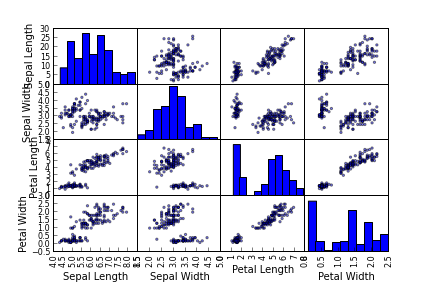
\includegraphics[height=8cm]{stat_cov_corr_01.png}

İlişki olduğu zaman o ilişkiye tekabül eden grafikte ``düz çizgiye benzer''
bir görüntü olur, demek ki değişkenlerden biri artınca öteki de artıyor
(eğer çizgi soldan sage yukarı doğru gidiyorsa), azalınca öteki de azalıyor
demektir (eğer çizgi aşağı doğru iniyorsa). Eğer ilinti yok ise bol
gürültülü, ya da yuvarlak küreye benzer bir şekil çıkar. Üstteki grafiğe
göre yaprak genişliği (petal width) ile yaprak boyu (petal length) arasında
bir ilişki var.

Tanım

$X,Y$ rasgele değişkenlerin arasındaki kovaryans,

$$ Cov(X,Y) = E(X-E(X))(Y-E(Y)) $$

Yani hem $X$ hem $Y$'nin beklentilerinden ne kadar saptıklarını her veri
ikilisi için, çıkartarak tespit ediyoruz, daha sonra bu farkları birbiriyle
çarpıyoruz, ve beklentisini alıyoruz (yani tüm olasılık üzerinden ne
olacağını hesaplıyoruz). 

Ayrı ayrı $X,Y$ değişkenleri yerine çok boyutlu $X$ kullanırsak, ki boyutları
$m,n$ olsun yani $m$ veri noktası ve $n$ boyut (özellik, öğe) var, tanımı şöyle
ifade edebiliriz,

$$ \Sigma = Cov(X) = E((X-E(X))^T(X-E(X))) $$

Phi Korelasyon Katsayısı

Phi katsayısı iki tane ikisel değişkenin birbiriyle ne kadar alakalı,
bağlantılı olduğunu hesaplayan bir ölçüttür. Mesela $x,y$ değişkenleri için
elde olan $(x_1,y_1),(x_2,y_2),..$ verilerini kullanarak hem $x=1$ hem
$y=1$ olan verileri sayıp toplamı $n_{11}$'e yazarız, $y=1,x=0$ icin
$n_{10}$, aynı şekilde diğer kombinasyonlara bakarak alttaki tabloyu
oluştururuz [5],

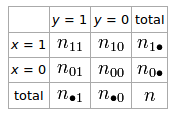
\includegraphics[width=12em]{phitable.png}

Phi korelasyon katsayısı

$$ 
\phi = \frac{n_{11}n - n_{1\bullet}n_{\bullet 1}}
{\sqrt{n_{0\bullet} n_{1\bullet} n_{\bullet 0} n_{\bullet 1}}} 
\mlabel{6}
$$

ile hesaplanır. Bu ifadeyi türetmek için iki rasgele değişken arasındaki
korelasyonu hesaplayan formül ile başlıyoruz,

$$ Corr(X,Y) = \frac{E (x-E(X)) (y-E(Y)) }{\sqrt{Var(X) \cdot Var(Y) } } $$

$$ 
= \frac{E(XY) - E(X)E(Y)}{ \sqrt{Var(X) \cdot Var(Y)} }
$$

$X,Y$ değişkenlerinin Bernoulli dağılımına sahip olduğunu düşünelim, çünkü
0/1 değerlerine sahip olabilen ikisel değişkenler bunlar, o zaman

$$
E[X]= \frac{n_{1\bullet}}{n}, \quad
Var[X]= \frac{n_{0\bullet}n_{1\bullet}}{n^2}, \quad
E[Y]= \frac{n_{\bullet 1}}{n}, \quad
Var[Y]= \frac{n_{\bullet 0}n_{\bullet 1}}{n^2}, \quad
E[XY]= \frac{n_{11}}{n^2}
$$

olacaktır. $E(XY)$ nasıl hesaplandı? Ayrıksal dağılımlar için beklenti
formülünün iki değişken için şöyle ifade edildiğini biliyoruz,

$$  E[XY] = \sum_i\sum_j x_i\cdot y_j \cdot P\{X = x_i, Y = y_j\} $$

Bu ifadeyi tabloya uyarlarsak, ve tablodaki hesapların üstteki ifadeler
için tahmin ediciler olduğunu biliyoruz, iki üstteki sonucu elde
edebileceğimizi görürüz, çünkü tek geçerli toplam $x_i y_i$ her iki
değişken de aynı anda 1 olduğunda geçerlidir. Bu değerleri yerine geçirince
(6) elde edilir.

Phi katsayısının bir diğer ismi Matthews korelasyon katsayısı. Bu hesabı
mesela bir 0/1 tahmini üreten sınıflayıcının başarısını ölçmek için
kullanabiliriz, gerçek, test 0/1 verileri bir dizinde, üretilen tahminler
bir diğerinde olur, ve Phi katsayısı ile aradaki uyumu raporlarız. Sonuç
-1,+1 arasında olacağı için sonuca bakarak irdeleme yapmak kolaydır, bu bir
başarı raporu olarak algılanabilir. Ayrıca Phi hesabının, AUC hesabı gibi,
dengesiz veri setleri üzerinde (mesela 0'a kıyasla çok daha fazla 1 olan
veriler, ya da tam tersi) üzerinde bile hala optimal olarak çalıştığı [4]
bulunmuştur.

Bazı örnekler,

\begin{minted}[fontsize=\footnotesize]{python}
from sklearn.metrics import matthews_corrcoef
y_true = [+1, +1, +1, -1]
y_pred = [+1, -1, +1, +1]
print (matthews_corrcoef(y_true, y_pred)  )
\end{minted}

\begin{verbatim}
-0.333333333333
\end{verbatim}

Ya da

\begin{minted}[fontsize=\footnotesize]{python}
a = [[0,  0],[0,  0],[0,  0],[0,  0],[0,  0],[1,  0],\
[1,  0],[1,  0],[0,  1],[0,  1],[1,  1],[1,  1],\
[1,  1],[1,  1],[1,  1],[1,  1],[1,  1],[1,  1],\
[1,  1], [1,  1],[1,  1],[1,  1],[1,  1],[1,  1],\
[1,  1],[1,  1],[1,  1]]
a = np.array(a)
print (matthews_corrcoef(a[:,0], a[:,1]))
\end{minted}

\begin{verbatim}
0.541553390893
\end{verbatim}

Medyan ve Yüzdelikler (Percentile)

Üstteki hesapların çoğu sayıları toplayıp, bölmek üzerinden yapıldı. Medyan
ve diğer yüzdeliklerin hesabı (ki medyan 50. yüzdeliğe tekabül eder) için
eldeki tüm değerleri "sıraya dizmemiz" ve sonra 50. yüzdelik için
ortadakine bakmamız gerekiyor. Mesela eğer ilk 5. yüzdeliği arıyorsak ve
elimizde 80 tane değer var ise, baştan 4. sayıya / vektör hücresine / öğeye
bakmamız gerekiyor. Eğer 100 eleman var ise, 5. sayıya bakmamız gerekiyor,
vs.

Bu sıraya dizme işlemi kritik. Kıyasla ortalama hesabı hangi sırada olursa
olsun, sayıları birbirine topluyor ve sonra bölüyor. Zaten ortalama ve
sapmanın istatistikte daha çok kullanılmasının tarihi sebebi de aslında bu;
bilgisayar öncesi çağda sayıları sıralamak (sorting) zor bir işti. Bu
sebeple hangi sırada olursa olsun, toplayıp, bölerek hesaplanabilecek
özetler daha makbuldü. Fakat artık sıralama işlemi kolay, ve veri setleri
her zaman tek tepeli, simetrik olmayabiliyor. Örnek veri seti olarak ünlü
\verb!dellstore2! tabanındaki satış miktarları kullanırsak,

\begin{minted}[fontsize=\footnotesize]{python}
print np.mean(data)
\end{minted}

\begin{verbatim}
213.948899167
\end{verbatim}

\begin{minted}[fontsize=\footnotesize]{python}
print np.median(data)
\end{minted}

\begin{verbatim}
214.06
\end{verbatim}

\begin{minted}[fontsize=\footnotesize]{python}
print np.std(data)
\end{minted}

\begin{verbatim}
125.118481954
\end{verbatim}

\begin{minted}[fontsize=\footnotesize]{python}
  print np.mean(data)+2*np.std(data)
\end{minted}

\begin{verbatim}
464.185863074
\end{verbatim}

\begin{minted}[fontsize=\footnotesize]{python}
print np.percentile(data, 95)
\end{minted}

\begin{verbatim}
410.4115
\end{verbatim}

Görüldüğü gibi üç nokta hesabı için ortalamadan iki sapma ötesini
kullanırsak, 464.18, fakat 95. yüzdeliği kullanırsak 410.41 elde
ediyoruz. Niye? Sebep ortalamanın kendisi hesaplanırken çok üç
değerlerin toplama dahil edilmiş olması ve bu durum, ortalamanın
kendisini daha büyük seviyeye doğru itiyor. Yüzdelik hesabı ise sadece
sayıları sıralayıp belli bazı elemanları otomatik olarak üç nokta
olarak addediyor.

Grupların Ortalamalarını ve Varyanslarını Birleştirmek

Bazen elimizde bir verinin farklı parçaları üzerinde hesaplanmış ortalama,
varyans sonucu olabilir, ve bu hesapları bu parçaların toplamı için
birleştirmemiz gerekebilir. Belki paralel süreçler var, verinin parçaları
üzerinde eşzamanlı çalışıyorlar, bir ortalama, varyans hesaplıyorlar,
ve nihai sonucun bu alt sonuçlar üzerinden raporlanması lazım [3].

İşlenen veri setinin tamamı, birleşmiş (pooled) veri $D = \{ x_1, x_2,.., x_N\}$ 
olsun, ki $N$ veri noktası sayısı. Bu verinin ortalaması $a = (x_1 + x_2 + .. + x_N) / N$, 
varyansı $v = ((x_1 - a)^2 + (x_2 - a)^2 + ... + (x_N - a)^2 ) / N$.  
Standart sapma tabii ki $\sigma_N = \sqrt{v}$.

Veriyi ayrı işledik diyelim, veri şu şekilde ayrıldı $D_1 = \{ x_1, x_2,..,x_j\}$,
$D_2 = \{ x_{j+1}, x_{j+2},..,x_{j+k}\}$, $D_3 = \{ x_{j+k+1}, x_{j+k+2},..,x_{j+k+m}\}$.
Yani her veri grubunun büyüklüğü sırasıyla $j,k,m$ ve toplam veri noktaları
$n = j+k+m$.

$D_P$'nin ortalaması $a_P = \frac{1}{n} \sum _{i=1}^{n} x_i$. Her grup $D_1,D_2,D_3$'un
ortalaması $a_1,a_2,a_3$ benzer şekilde bulunabilir. Bu durumda ``ortalamaların
ortalaması'', yani nihai ortalama $a_P$ şöyle bulunabilir,

$$
a_P = (j a_1 + k a_2 + m a_3 ) / n
$$

Varyansa ulaşmak için kareler toplamı, grup varyanslarına bakalım şimdi, $D_P$
için kareler toplamı

$$
S_P = \sum _{i=1}^{n} x_i^2
\mlabel{7}
$$

Gruplar $D_1,D_2,D_3$ için toplamlar $S_1,S_2,S_3$ benzer şekilde tanımlanıyor,
ve nihai toplam bu gruplar üzerinden $S_P = S_1 + S_2 + S_3$ olarak
tanımlanabiliyor.

Tum veri $D_P$ icin varyans

$$
v_P = \frac{1}{n} \sum_{i=1}^{n} (x_i - a_P)^2
$$

Bu ifadeyi acarsak

$$
= \frac{1}{n} \sum_{i=1}^{n} ( x_i^2 - 2 x_i a_p + a_p^2 )
$$

$$
= \frac{1}{n} \sum_{i=1}^{n}  x_i^2  - \frac{1}{n} \sum_{i=1}^{n}  2 x_i a_p + \frac{1}{n} \sum_{i=1}^{n} a_p^2
$$

$\frac{1}{n} \sum_{i=1}^{n} x_i = a_p$ olduğunu hatırlarsak, ve $\frac{1}{n} \sum_{i=1}^{n} a_p$
tabii ki yine $a_p$ o zaman 

$$
= S_p / n  - 2 a_p^2 + \frac{1}{n} \sum_{i=1}^{n} a_p^2
$$

$\frac{1}{n} \sum_{i=1}^{n} a_p^2$ benzer sekilde tekrar $a_p$, 

$$
= S_p / n  - 2 a_p^2 +  a_p^2
$$

$$
v_P = S_p / n  -  a_p^2
\mlabel{8}
$$

Bu durumda parçaların ayrı varyans formülleri de üstteki gibi yazılabilir,

$$
v_1 = S_1 / j  -  a_1^2, \quad
v_2 = S_2 / k  -  a_2^2, \quad
v_3 = S_3 / m  -  a_3^2
\mlabel{9}
$$

Amacımız $v_p$'yi ufak parçaların varyansları $v_1,v_2,v_3$ üzerinden hesaplamak.

Simdi (7,8,9) formullerini kullanarak $v_p$ su sekilde de yazilabilirdi,

$$
v_p = (S_1 + S_2 + S_3) / n
$$

Ya da

$$
n v_p = S_1 + S_2 + S_3 - n a_p^2
$$

Açarsak

$$
n v_p = j (v_1 + a_1)^2 + k (v_2 + a_2)^2 + m (v_3 + a_3)^2 - n a_p^2
\mlabel{10}
$$

Şu da söylenebilir,

$$
n v_p = j v_1 + k v_2 + m v_3 + j a_1^2 + k a_2^2 + m a_3^2 - n a_p^2
$$

Şimdi (10) formülüne nasıl erisebileceğimizi düşünelim. Alttaki iki kavramdan
hareketle bunu yapabilir miyiz acaba?

Varyansların ortalamasını

$$
a_v = (j v_1 + k v_2 + m v_3) / n
$$

ve ortalamaların varyansını

$$
v_a = [ j(a_1-a_p)^2 + k(a_2-a_p)^2 + m(a_3-a_p)^2 ] / n
$$

diye tanımlayalım. Üstteki formülü açalım,

$$
n v_a = j(a_1-a_p)^2 + k(a_2-a_p)^2 + m(a_3-a_p)^2 
$$

$$
= j a_1^2 + k a_2^2 + m a_3^2 - 2 a_p (ja_1 + ka_2 + ma_3) + n a_p^2
$$


Box Whisker Grafikleri

Tek boyutlu bir verinin dağılımını görmek için Box ve Whisker grafikleri
faydalı araçlardır; medyan (median), dağılımın genişliğini ve sıradışı
noktaları (outliers) açık şekilde gösterirler. İsim nereden geliyor? Box
yani kutu, dağılımın ağırlığının nerede olduğunu gösterir, medyanın
sağındada ve solunda olmak üzere iki çeyreğin arasındaki kısımdır, kutu
olarak resmedilir. Whiskers kedilerin bıyıklarına verilen isimdir, zaten
grafikte birazcık bıyık gibi duruyorlar. Bu uzantılar medyan noktasından
her iki yana kutunun iki katı kadar uzatılır sonra verideki "ondan az olan
en büyük" noktaya kadar geri çekilir. Tüm bunların dışında kalan veri ise
teker teker nokta olarak grafikte basılır. Bunlar sıradışı (outlier)
oldukları için daha az olacakları tahmin edilir.

BW grafikleri iki veriyi dağılımsal olarak karşılaştırmak için

içeren Quintus Curtius Snodgrass veri setinin değişik olduğunu
ispatlamak için bir sürü hesap yapmışlardır, bir sürü matematiksel
işleme girmişlerdir, fakat basit bir BW grafiği iki setin farklılığını
hemen gösterir.

BW grafikleri iki veriyi dağılımsal olarak karşılaştırmak için
birebirdir. Mesela Larsen and Marx adlı araştırmacılar çok az veri
içeren Quintus Curtius Snodgrass veri setinin değişik olduğunu
ispatlamak için bir sürü hesap yapmışlardır, bir sürü matematiksel
işleme girmişlerdir, fakat basit bir BW grafiği iki setin farklılığını
hemen gösterir.

Python üzerinde basit bir BW grafiği 

\begin{minted}[fontsize=\footnotesize]{python}
spread= rand(50) * 100
center = ones(25) * 50
flier_high = rand(10) * 100 + 100
flier_low = rand(10) * -100
data =concatenate((spread, center, flier_high, flier_low), 0)
plt.boxplot(data)
plt.savefig('stat_feat_01.png')
\end{minted}

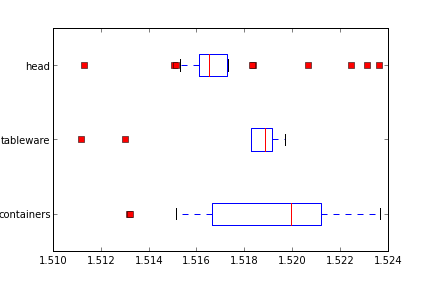
\includegraphics[height=6cm]{stat_feat_01.png}

Bir diğer örnek Glass veri seti üzerinde

\begin{minted}[fontsize=\footnotesize]{python}
data = loadtxt("glass.data",delimiter=",")
head = data[data[:,10]==7]
tableware = data[data[:,10]==6]
containers = data[data[:,10]==5]

print head[:,1]

data =(containers[:,1], tableware[:,1], head[:,1])

plt.yticks([1, 2, 3], ['containers', 'tableware', 'head'])

plt.boxplot(data,0,'rs',0,0.75)
plt.savefig('stat_feat_02.png')
\end{minted}

\begin{verbatim}
[ 1.51131  1.51838  1.52315  1.52247  1.52365  1.51613  1.51602  1.51623
  1.51719  1.51683  1.51545  1.51556  1.51727  1.51531  1.51609  1.51508
  1.51653  1.51514  1.51658  1.51617  1.51732  1.51645  1.51831  1.5164
  1.51623  1.51685  1.52065  1.51651  1.51711]
\end{verbatim}

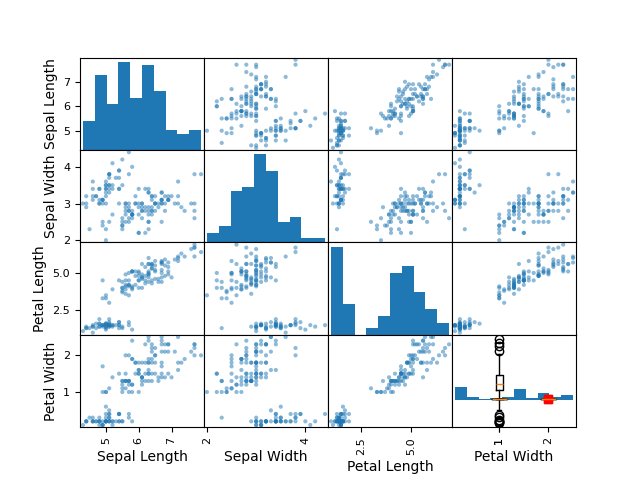
\includegraphics[height=6cm]{stat_feat_02.png}

Kaynaklar

[1] Ross, {\em Introduction to Probability and Statistics for Engineers, 3rd Edition}

[2] Wasserman, {\em All of Statistics}

[3] Rudmin, {\em Calculating the Exact Pooled Variance},
    \url{https://arxiv.org/abs/1007.1012}

[4] Boughorbel, {\em Optimal classifier for imbalanced data using Matthews Correlation Coefficient metric}, \url{http://journals.plos.org/plosone/article/file?id=10.1371/journal.pone.0177678&type=printable}

[5] Cross Validated, {\em Relation between the phi, Matthews and Pearson correlation coefficients?}, \url{https://stats.stackexchange.com/questions/59343/relation-between-the-phi-matthews-and-pearson-correlation-coefficients}

[6] Bayramli, Diferansiyel Denklemler, {\em Ters Trigonometrik Formüller}

\end{document}
